\documentclass{beamer}
%\documentclass[notes=show]{beamer}

\usepackage[utf8]{inputenc}
\usepackage[german]{babel}
\usepackage{rotating}

\usepackage{german, latexsym}
\usepackage{floatflt}
\usepackage{graphicx}
%\definecolor{lightblue}{rgb}{0.8,0.9,1.0}
%\usetheme{PaloAlto}
%\usetheme{Darmstadt}
\usetheme{Frankfurt}
%\usetheme{Berlin}

%\usecolortheme{crane}
%\usecolortheme{wolverine}
\usecolortheme{seagull}
%\usecolortheme{albatross}
%\usecolortheme{beetle}
%\usecolortheme{lily}

\usepackage{pgf,pgfarrows,pgfnodes,pgfautomata,pgfheaps}
\usepackage{amsmath,amssymb}

\setbeamercovered{dynamic}


%notes:
\setbeamertemplate{note page}[plain] 
%compressed

\title[]{  Simulation paralleler E/A auf Anwendungs- und Systemebene }
\author{ \underline{Julian M. Kunkel} } %Research Group:
\institute{ Institut für Informatik \\  Parallele und Verteilte Systeme \\ Ruprecht-Karls-Universit\"at Heidelberg}
\date{  27.09.2009 }
\beamertemplatetransparentcovereddynamic
\setbeamerfont{note page}{size=\small}
%\setbeamersize{text margin left=0.1cm,text margin right=0.1cm}
%\renewcommand{\>}{\rangle}
%\newcommand{\<}{\langle} 
%\usebeamercolor[fg]{[page number]}

\setbeamertemplate{navigation symbols}{}
%\setbeamertemplate{note page}{}

\setbeamersize{text margin left=0.2cm}
\setbeamersize{text margin right=0.2cm}
\setbeamersize{sidebar width right=0cm}
\setbeamersize{sidebar width left=0cm}

\setbeamertemplate{footline}
{
\begin{beamercolorbox}{title}
\hspace*{0.2cm}
% \copyright 
Julian M. Kunkel 
\hfill
 \insertslidenavigationsymbol
 \insertframenavigationsymbol
 \insertsubsectionnavigationsymbol
 \insertsectionnavigationsymbol
 \insertdocnavigationsymbol
 \insertbackfindforwardnavigationsymbol
 \hfill\insertframenumber/\inserttotalframenumber
 \hspace*{0.2cm}
\end{beamercolorbox}
}

%\newcommand{\markNote}[1]{	\textsuperscript{\tiny [#1]} }
\newcommand{\markNote}[1]{	 }

%\AtBeginSection[]{
%\frame{
      %\frametitle{Outline}
	%\tableofcontents[current,hideallsubsections]
%	}
%}

\begin{document}
\frame{
	\titlepage
}

\frame{
\frametitle{Agenda}
\tableofcontents[hideallsubsections]
}

\newcommand {\myframe}[2]{
\frame{
	\frametitle{#1} 
	\begin{itemize}
	#2 
	\end{itemize}
}
}

\newcommand {\itemm}[1]{
  	\begin{itemize}
	\item #1
	\end{itemize}
}

\section{Ziele}

\myframe{Ziele}{
\item MPI and MPI-IO Befehle simulieren
  \itemm{Abschätzung für Effizienz einer Implementierung}
\item Einfache Modelle für Hardware und Software
\item Konfiguration der Hardware/Software nach belieben
  \itemm{Schätze Skalierbarkeit von Software in beliebigen Cluster Umgebungen}
\item Einsatz/Nutzbarmachung von Standard-Tools zur Analyse
  \itemm{Simulationsergebnisse genau wie realle Programläufe bewerten}
\item Neue Algorithmen/Verhalten schnell und reproduzierbar testen
\item Einsetzbarkeit für Lehre
   \itemm{Soll auf Desktop PC lauffähig sein}
}

\section{Hardware Model}
\subsection{Hardware Modell}
\myframe{Hardware Modell}{
\item Komponententypen an existierende Hardware angelehnt\\ z.B. “Knoten” oder “I/O-subsystem”
\item Je Komponententyp sind alternative Implementierungen möglich\\ z.B. SSD oder Disk
\item Cluster Modell beschreibt konkrete Implementierungen der Komponenten und Charakteristika
\item Deterministisches Komponentenverhalten
}

\subsection{Simulierte Komponenten}
\frame{
  \frametitle{Simulierte Komponenten}
  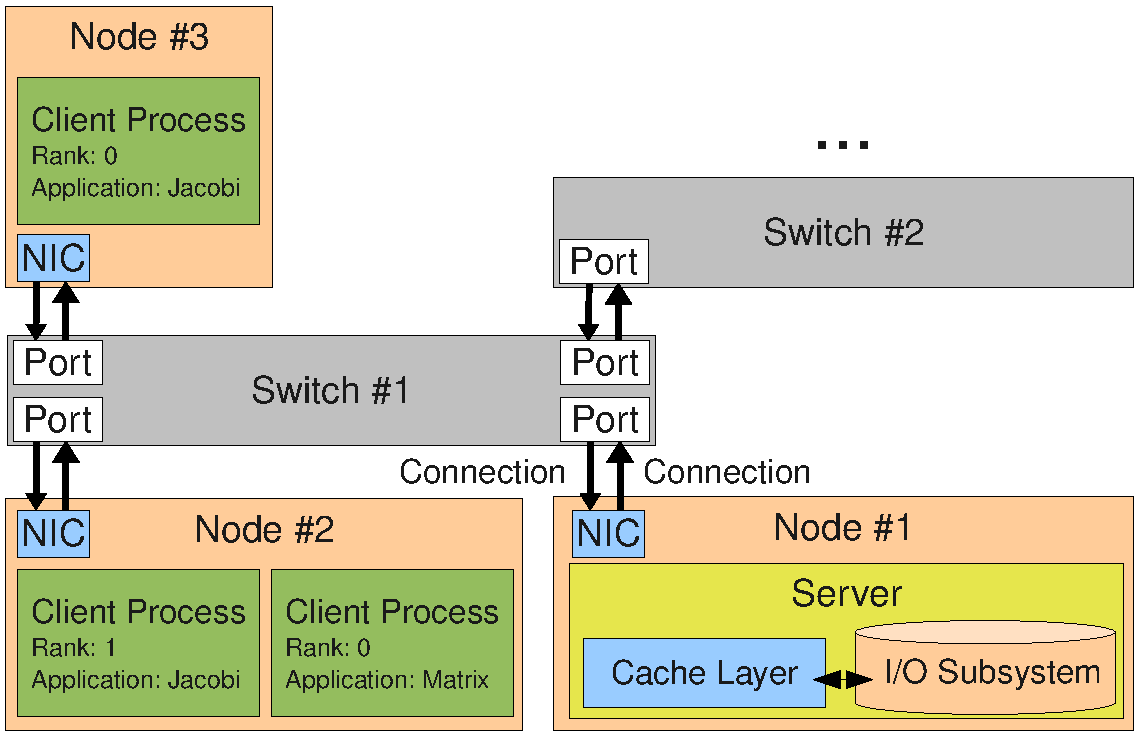
\includegraphics[width=0.95\textwidth]{Simulator-Components.pdf}
}

\subsection{Hardware Model - Charakteristika}
\myframe{Hardware Model - Charakteristika}{
\item Knoten:
  \itemm{\# CPUs, Abarbeitungsgeschwindigkeit}
\item Netzwerkkarte:
  \itemm{Latenz, Durchsatz}
\item Server Cache Layer - Caching von I/O Daten, steuert I/O Subsystem
\itemm{Cache Größe}
\item I/O Subsystem:
\itemm {Je nach Datei und letztem Offset wird die Zugriffszeit ermittelt
    \item Track-To-Track Zugriffzeit, Mittlere Zugriffszeit}
\item Switch:
  \itemm{Store-and-Forward Switching
  \item Besteht aus N-Ports}
\item Port:
  \itemm{Latenz, Durchsatz}
}

\subsection{Datenfluss Model}
\myframe{Datenfluss Model}{
  \item Datenflüsse als Flüsse von Paketen
  \item Eine Netzwerkkomponente kann eine Menge von Paketen transferieren 
  \itemm{Bis das Kabel mit Daten saturiert ist
    \item Der weitere Datenfluss wird dann blockiert} 
  %\item Alternative Anschauung: wenn mindestens soviele Daten unterwegs sind um die Latenz zu überbrücken 
  \item Bei Bearbeitung eines Pakets wird der Sender benachrichtigt
    \itemm{Diese darf nun weitere Pakete transferieren 
    \item Kaskade von nachrückenden Paketen kann aktiviert werden}
  \item Es wird ein Fluss pro Ziel nach obigem Schema verwaltet
   \itemm{Engpässe die in Flussrichtung auftreten blockieren nicht den Transfer an andere Adressen
     \item Anschaulich: ein Switch verwaltet pro Netzwerkadresse eine Warteschlange mit fester Länge
    }
  \item Server können Datenflüsse aktiv blockieren z.B. bei gefülltem I/O Cache 
  \item Datenfluss Model ist an Realität angelehnt garantiert aber optimalen Transfer (unter gegegebenem Paketmaximum) 
  \item Überholvorgänge innerhalb des Netzwerks sind nicht möglich
  \item Gegenwärtig nur eine Route
} 

\section{Software Model}
\subsection{Software Model}
\myframe{Software Model}{
\item Anwendung 
\itemm{MPI Semantik
  \item Nichtblockierende Operationen werden unterstützt
  \item Rechenoperationen werden nur durch eine Dauer charakterisiert
  \item Gleichmäßige Zuteilung der CPU Ressourcen zu Rechenjobs}
  
\item Mehrere (MPI-IO) Anwendungen können gleichzeitig gestartet werden  
  \itemm{Insbesondere im I/O-Subsystem ist ein anderes Lastverhalten zu erwarten}
}

\subsection{Modellierung von MPI Befehlen}
\myframe{Modellierung von MPI Befehlen}{
  \item Algorithmen sind austauschbar
  \itemm{Bei Ausführung Algorithmus spezifizieren}
\item Abarbeitung in endlichen Automaten
  \itemm{Programmierung der Zustände
    \item Existierende Befehle können aufgerufen werden
    \item Netzwerkoperationen 
    \item (Eigenverwaltete) Blockierung möglich}
\item Globale Sicht auf alle Prozesse 
  \itemm{Metawissen soll programmierung von einem Best-Case erlauben
    \item Ermöglicht bspw. “Virtuelle” Bariere}
}

\section{Implementierung}
\myframe{Implementierung des Simulators}{
  \item Java (Version 5)
  \item GPL
  \item Sequenzieller Code
  \item Schreibt TAU-Trace oder HDTrace zur Analyse
  \begin{block}{Diskrete Ereignis-Simulation}
  Solange Ereignisse vorhanden sind:
  \itemm{    
    Bearbeite (ein) frühestes Ereignis durch delegation an die entsprechende Komponente
    \item Erzeugt ggf. weitere Ereignisse in der Zukunft
    }
  \end{block}

\begin{block}{Jobs}
    \begin{itemize}
     \item Operationen die von einer Komponente exklusiv bearbeitet werden
     \item Beispiel: Datenpakete
     \item Start und Ende Ereignis
     \item Bearbeitung von Jobs wird von Komponente Verwaltet und erfolgt in FIFO
    \end{itemize}   
  \end{block}
}

\section{Ergebnisse}
\subsection{Validierung des Simulators}
\myframe{Validierung des Simulators}{
 \item Existierender Program getraced und simuliert
 \item Jacobi Verfahren - PDE: Iterative Lösung der Poisson Gleichung
 \itemm{
 100 Iterationen
 \item Master Prozess sammelt Ergebnisse ein
 \item Keine I/O 
 }
 \item Cluster Model analog zu unserem 10 Knoten (Test-)Cluster
}

\frame{
  \frametitle{Jacobi - PDE}
   
\begin{table}
\begin{center}
\begin{tabular}{l||l|l|l}
Prozessanzahl & Laufzeit in s & Simulierte Laufzeit & Simuliert/Real \\
\hline
\hline
1 & 47.30 & 47.35 & 1.001 \\
2 & 24.79 & 24.93 & 1.006 \\
3 & 17.3 & 17.54 & 1.014 \\
4 & 13.54 & 13.75 & 1.016 \\
5 & 11.56 & 11.82 & 1.022 \\
6 & 10.09 & 10.33 & 1.024 \\
7 & 9.16 & 9.44 & 1.030 \\
8 & 8.39 & 8.73 & 1.041 \\
9 & 8.00 & 8.26 & 1.033
\end{tabular}
\end{center}
\end{table}

}

\subsection{I/O Optimierungen}

\myframe{I/O Optimierungen}{
  \begin{block}{Ziele}
  \item Effizienz verschiedener Optimierungen soll überprüft werden
  \item Kollektive Optimierungen - Two-Phase* vs. Serverseitige Optimierungen
  \item Entwicklung neuer I/O Optimierungsstrategien
  \end{block}
  
  \begin{block}{Server-Directed I/O}
  \begin{itemize}
  \item Cache-Optimierungsstrategie auf I/O Servern
  \item Datentransfer zwischen Client/Server wird durch Server bestimmt
  \item Interessant für nichtzusammenhängende Zugriffe
  \itemm{Cache-Schicht bestimmt welche Daten mit Client ausgetauscht werden sollen
    \item Im Moment für Lesezugriffe implementiert
    \item Reads aller ausstehenden Anfragen sind bekannt
    \item Priorisiere große zusammenhängende Reads}
  
  \end{itemize}  
  \end{block}
}

\myframe{}{
  \item 
}


%Kritische Betrachtungen
%Interface für (Hardware) Komponenten teilweise schwer definierbar
%Hängt von Hardware Eigenschaften ab
%Gegenwärtig werden Interfaces nach Anforderungen erweitert
%Server Cache Layer aber soweit fest

\section{Fazit}
\myframe{Fazit}{
  \item Einfaches Model für Simulation von MPI und Cluster Hardware
  \item Geeignet für Simulation von heterogenen Umgebungen und Netztopologien
  \item Testen von alternativen Implementierungen für MPI Befehle
  \item Verschiedene I/O Optimierungen wurden evaluiert
  \item Server-Seitige Optimierung in den meisten Fällen ausreichend
}


\section{Angelehnte Projekte}

\subsection{Tracing}
\frame{
  \begin{block}{}
  \centering
  Tracing Umgebung
  \end{block}
}

\myframe{Tracing}{
\item Existierende Formate stellten nicht genügend Information bereit
\itemm{Simulator benötigt alle Parameter eines MPI Aufrufs
  \item Nichtzusammenhängende I/O muss gespeichert werden}
\item Eigene Tracing Umgebung
\itemm{
  Trace Format(e)
  \item MPIWrapper
  \item Viewer
  }
}

\subsection{Simulation von Energiesparstrategien}

\frame{
  \begin{block}{}
  \centering
  Simulation von Energiesparstrategien
  \end{block}
}

\myframe{Ziele}{
  \item Vergleiche (simulierten) Energieverbrauch der Anwendung mit verschiedenen Sparstrategien
  \item Berechne minimale Energiekosten bei optimal (energiesparenden) Komponenten
  \itemm{d.h. Energieverbrauch ist proportional zur Leistung 
    \item Obere Schranke für Energieeinsparpotenzial 
  }
  \item Strategien könnten auch (bedingt) Umstrukturierung des Programs berücksichtigen
  \itemm{bspw. verzögern von Netzwerk und I/O Aktivität}
  \item Anwendbarkeit bei beliebigen Programmen (auch Lokal)
}

\myframe{Simulation von Energiesparstrategien - Methodik}{  
  \item Tracing der Auslastung von CPU, Netwerk, I/O-subsystemen in festen Intervalen
  \item Verwende Auslastung der einzelnen Komponenten um Energieverbrauch zu schätzen  
  \itemm{Lineare Interpolierung des Energieverbrauchs (Max/Min) bei Auslastung}
  \itemm{ACPI Model für Energieverbrauch/Dauer eines Zustandwechsels}
  \item Strategien können künftige Zustände erkennen und Komponenten bei dieser Last bestmöglich steuern
  \itemm{Eine Umordung/Verschiebung der Last ist teilweise möglich}
  \item Vergleich der Simulierten Ergebnisse mit gemessenem Energieverbrauch
  \itemm{Ebenfalls eine Eichung des Models}
}

\myframe{Beispielstrategie - Approach Strategie}{
  \item Betrachte die Last der nächsten (zukünftigen) k-Intervalle
  \item Kosten Zustandswechsel und Aktivierung vs. Einsparungspotenzial
  \itemm{$\Rightarrow$ minimale Zeit in der es sich lohnt die Komponente in den sparsameren Zustand zu versetzen}
  \item Bei wenig Last $\le 10\%$  verzögere diese (wenn möglich) auf später
  \itemm{10 x 10\% resultiert in einem Zustand mit 100\% Last}
}

\myframe{Ergebnisse - Jacobi PDE}{
 \item Iterationen: 5 (rechen intensiv), 500 (kommunikations intensiv)
 \item Für I/O wurde jede Iteration ein Checkpointing auf PVFS gemacht
 \item Die Abweichung zwischen gemessener Leistungsaufnahme und Simulierter beträgt im Beispiel $\leq$ 3\%.
  \begin{table}
  \begin{center}
  \begin{tabular}{l||l|l|l|l}
  Konfiguration & Simple S. & Optimale S. & Approach S. & Eff. Geräte \\
  \hline
  \hline
  4 p/500 & 90\,Watt & 17\% & 19\% & 33\% \\
  4x2 p/500 & 70\,Watt & 2.3\% & 2.6\% & 9.3\% \\
  4 p/5 + I/O & 20\,Watt & 7\% & 11\% & 28\% \\
  4x2 p/5 + I/O & 18.5\,Watt & 4.7\% & 6.7\% & 23.5\% \\  
  \end{tabular}
  \end{center}
  \end{table}
  % 500 iterationen => 4 nodes x 2 prozesse
  % 5 iterationen
}

\myframe{Fazit}{
  \item Auslastung bestimmt Energieeffizienz
  \item Potenzial für Energieeinsparung vorhanden
  \item Simulation ist ein Ansatz für Berechnung
  \item Abschätzung für Energiekosten und Verlust durch Programme
}

\end{document}
